\documentclass[11pt,a4paper]{article}
\usepackage[utf8]{inputenc}
\usepackage[T1]{fontenc}
\usepackage{lmodern}
\usepackage[italian]{babel}
\usepackage[margin=2.2cm]{geometry}
\usepackage{graphicx}
\usepackage{booktabs}
\usepackage{amsmath}
\usepackage{float}
\usepackage[most]{tcolorbox}

\title{FM$^2$ su mappe casuali: FMM contro Block FIM al crescere della difficoltà}
\author{Carlo Barone}
\date{28 ottobre 2026}

\begin{document}
\maketitle

\section{Che cosa si è misurato}
Su molte mappe 3D generate a caso si è calcolato il FM$^2$ completo (passata 1, distanza dagli ostacoli, più passata 2, tempo di arrivo da B) con il Fast Marching Method sulla CPU e con il Block FIM sulla GPU, e se ne sono confrontati i tempi.

\paragraph{Stanza e mappe.} Cubo $[-1,1]^3$ (20 m di lato). $K$ muri spessi 0.1 (1 m) perpendicolari a $x$, equidistanti tra $x=-0.6$ e $x=0.6$; ogni muro ha $M$ fori quadrati di lato casuale e posizione casuale. A è a caso nel primo scomparto, B nell'ultimo. Ogni mappa è individuata da un \emph{seed} ($1000\cdot(\text{livello}-1)+$ numero della mappa): stesso seed, stessa mappa, anche su griglie diverse.

\begin{table}[H]
\centering
\begin{tabular}{cccc}
\toprule
livello & muri $K$ & fori per muro $M$ & lato dei fori \\
\midrule
1 & 2 & 3 & 0.30--0.50 (3--5 m) \\
2 & 3 & 2 & 0.25--0.45 \\
3 & 4 & 2 & 0.20--0.40 \\
4 & 5 & 2 & 0.15--0.35 \\
5 & 6 & 1 & 0.15--0.30 (1.5--3 m) \\
\bottomrule
\end{tabular}
\caption{I cinque livelli di difficoltà.}
\end{table}

\paragraph{Prove.} 30 mappe per livello a $N=129$ (150 mappe), 10 a $N=193$ (50), 2 a $N=257$ (10): \textbf{210 mappe} in tutto, in un'unica esecuzione su Google Colab (GPU NVIDIA Tesla T4, 40 multiprocessori). Parametri del FM$^2$ come negli altri notebook: \texttt{MARGINE} = 0.06, \texttt{D\_SICUREZZA} = 0.3, \texttt{V\_MIN} = 0.1; Block FIM con blocchi $8^3$, \texttt{niter} = 8, $\varepsilon = 10^{-6}$.

\paragraph{Tempi.} Il FMM è misurato una volta (dura da 0.3 a 7.6 s); il Block FIM tre volte, e si tiene il minimo. Il tempo del Block FIM è quello del ciclo dei giri (eventi CUDA), senza allocazione e copie tra CPU e GPU, come nelle altre tabelle. Speedup = $t_\text{FMM}/t_\text{Block FIM}$.

\section{Il risultato principale: come si comportano FMM e Block FIM al crescere del livello}
\begin{tcolorbox}[colback=blue!4,colframe=blue!50!black,title=In sintesi]
Salendo di livello (più muri, fori più piccoli e sfalsati) lo speedup del Block FIM sul FMM \textbf{cala}, ma \textbf{non perché il Block FIM rallenti}:
\begin{itemize}
  \item il \textbf{FMM diventa più veloce}, perché con più muri ci sono meno nodi liberi da calcolare;
  \item il \textbf{Block FIM resta quasi costante}: fa \textbf{più giri}, ma \textbf{ogni giro costa meno}, e i due effetti si compensano.
\end{itemize}
Lo speedup cala quindi perché il problema diventa più \emph{facile} per il FMM, non più \emph{difficile} per il Block FIM.
\end{tcolorbox}

\begin{table}[H]
\centering
\small
\begin{tabular}{c|c|c|ccc|c}
\toprule
 & nodi liberi & \textbf{FMM} & \multicolumn{3}{c|}{\textbf{Block FIM}} & \\
livello & ($\times 10^6$)$^{*}$ & tempo [ms] & giri & tempo per giro [$\mu$s] & tempo [ms] & speedup \\
\midrule
1 & 1.30 & 811 & 110 & 158 & 17.1 & 47.8 \\
2 & 1.11 & 656 & 131 & 136 & 17.7 & 36.8 \\
3 & 0.95 & 527 & 149 & 107 & 15.6 & 33.8 \\
4 & 0.75 & 406 & 159 & 100 & 15.8 & 25.9 \\
5 & 0.59 & 318 & 200 & 86 & 17.2 & 18.3 \\
\midrule
dal liv.~1 al liv.~5 & $-55\%$ & $\mathbf{-61\%}$ & $\mathbf{+82\%}$ & $\mathbf{-46\%}$ & $\mathbf{\approx 0\%}$ & $-62\%$ \\
\bottomrule
\end{tabular}
\caption{$N=129$, valori mediani su 30 mappe per livello. $^{*}$Nodi liberi della prima mappa di ogni livello (stesso seed, prova locale). A $N=257$ (2 mappe per livello) l'andamento è lo stesso: FMM da 7500 a 2414 ms ($-68\%$), giri da 208 a 428 ($+106\%$), tempo per giro da 345 a 120 $\mu$s ($-65\%$), Block FIM da 71 a 51 ms ($-28\%$).}
\end{table}

\begin{figure}[H]
\centering
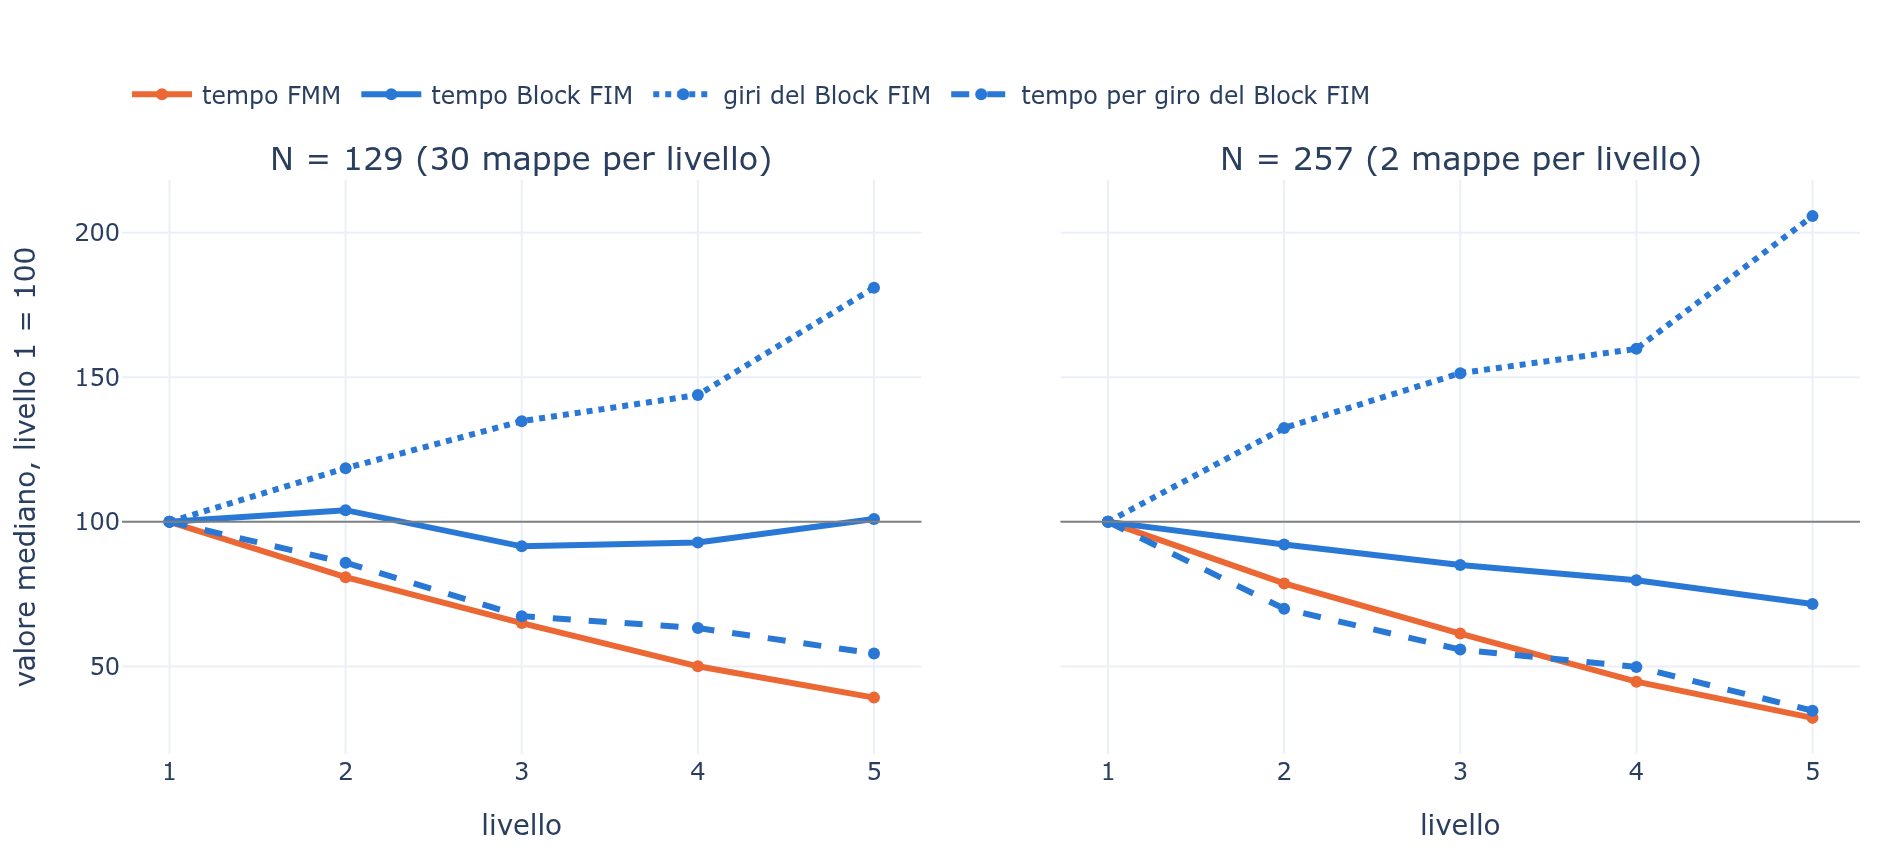
\includegraphics[width=\textwidth]{fig_confronto.png}
\caption{Andamento con il livello, rispetto al livello 1 (= 100). Arancione: tempo del FMM. Blu: tempo del Block FIM (linea continua), suoi giri (punti) e tempo per giro (tratteggio). I giri salgono, il tempo per giro scende, il tempo totale del Block FIM resta circa piatto; il tempo del FMM scende con i nodi liberi.}
\end{figure}

\paragraph{Perché il FMM accelera.} Il FMM tratta ogni nodo libero una volta, estraendolo dalla coda ordinata: il suo costo dipende quasi solo dal numero di nodi liberi, non dalla forma del percorso. I muri tolgono nodi (da $1.30$ a $0.59$ milioni a $N=129$) e il tempo scende in proporzione.

\paragraph{Perché il Block FIM no.} Il Block FIM procede a giri: a ogni giro lavora in parallelo su tutti i blocchi attivi. Con più muri e fori sfalsati il fronte deve girare attorno agli ostacoli e i blocchi vengono riattivati più volte, quindi servono \textbf{più giri}. Ma a ogni giro i blocchi attivi sono \textbf{pochi} (il fronte passa per fori stretti) e il giro costa meno. Più giri per meno lavoro a giro: il tempo totale resta circa lo stesso. Il costo del Block FIM dipende quindi soprattutto da quanto è \emph{tortuoso} il percorso del fronte (i giri), mentre quello del FMM dal \emph{numero di nodi}.

\section{Risultati}
\begin{table}[H]
\centering
\small
\begin{tabular}{ccc|cc|c|cc|c|c}
\toprule
$N$ & liv. & mappe & \multicolumn{2}{c|}{speedup} & giri & $t_\text{FMM}$ & $t_\text{BFIM}$ & volo & max \\
 & & & mediano & min--max & mediani & [ms] & [ms] & [s] & $|\text{FMM}-\text{BFIM}|$ \\
\midrule
129 & 1 & 30 & 47.8 & 37.0--64.7 & 110 & 811 & 17.1 & 23 & 9.5e$-$6 \\
129 & 2 & 30 & 36.8 & 32.4--42.3 & 131 & 656 & 17.7 & 35 & 1.4e$-$5 \\
129 & 3 & 30 & 33.8 & 29.1--39.8 & 149 & 527 & 15.6 & 52 & 1.8e$-$5 \\
129 & 4 & 30 & 25.9 & 21.8--30.9 & 159 & 406 & 15.8 & 86 & 3.0e$-$5 \\
129 & 5 & 30 & 18.3 & 15.4--23.4 & 200 & 318 & 17.2 & 185 & 8.4e$-$5 \\
\midrule
193 & 1 & 10 & 85.3 & 71.7--92.0 & 161 & 2904 & 33.7 & 23 & 1.2e$-$5 \\
193 & 2 & 10 & 75.4 & 70.3--83.0 & 200 & 2437 & 32.1 & 37 & 2.0e$-$5 \\
193 & 3 & 10 & 59.8 & 54.1--66.4 & 217 & 1891 & 31.3 & 49 & 2.7e$-$5 \\
193 & 4 & 10 & 46.8 & 42.1--57.7 & 240 & 1426 & 30.3 & 81 & 4.6e$-$5 \\
193 & 5 & 10 & 34.3 & 30.7--39.7 & 324 & 1019 & 30.4 & 209 & 1.1e$-$4 \\
\midrule
257 & 1 & 2 & 105.2 & 103.6--106.7 & 208 & 7500 & 71.3 & 22 & 1.4e$-$5 \\
257 & 2 & 2 & 90.0 & 86.7--93.2 & 276 & 5904 & 65.7 & 40 & 1.8e$-$5 \\
257 & 3 & 2 & 75.9 & 74.0--77.8 & 315 & 4600 & 60.7 & 62 & 2.3e$-$5 \\
257 & 4 & 2 & 59.0 & 56.8--61.2 & 332 & 3354 & 56.9 & 85 & 4.8e$-$5 \\
257 & 5 & 2 & 47.4 & 46.6--48.1 & 428 & 2414 & 51.0 & 211 & 9.2e$-$5 \\
\bottomrule
\end{tabular}
\caption{Valori mediani per griglia e livello. ``Volo'' = $u(A)\times 5$ s (1 unità = 10 m, velocità massima 2 m/s). L'ultima colonna è la differenza massima tra le due $u$ su tutte le mappe del gruppo.}
\end{table}

\begin{figure}[H]
\centering
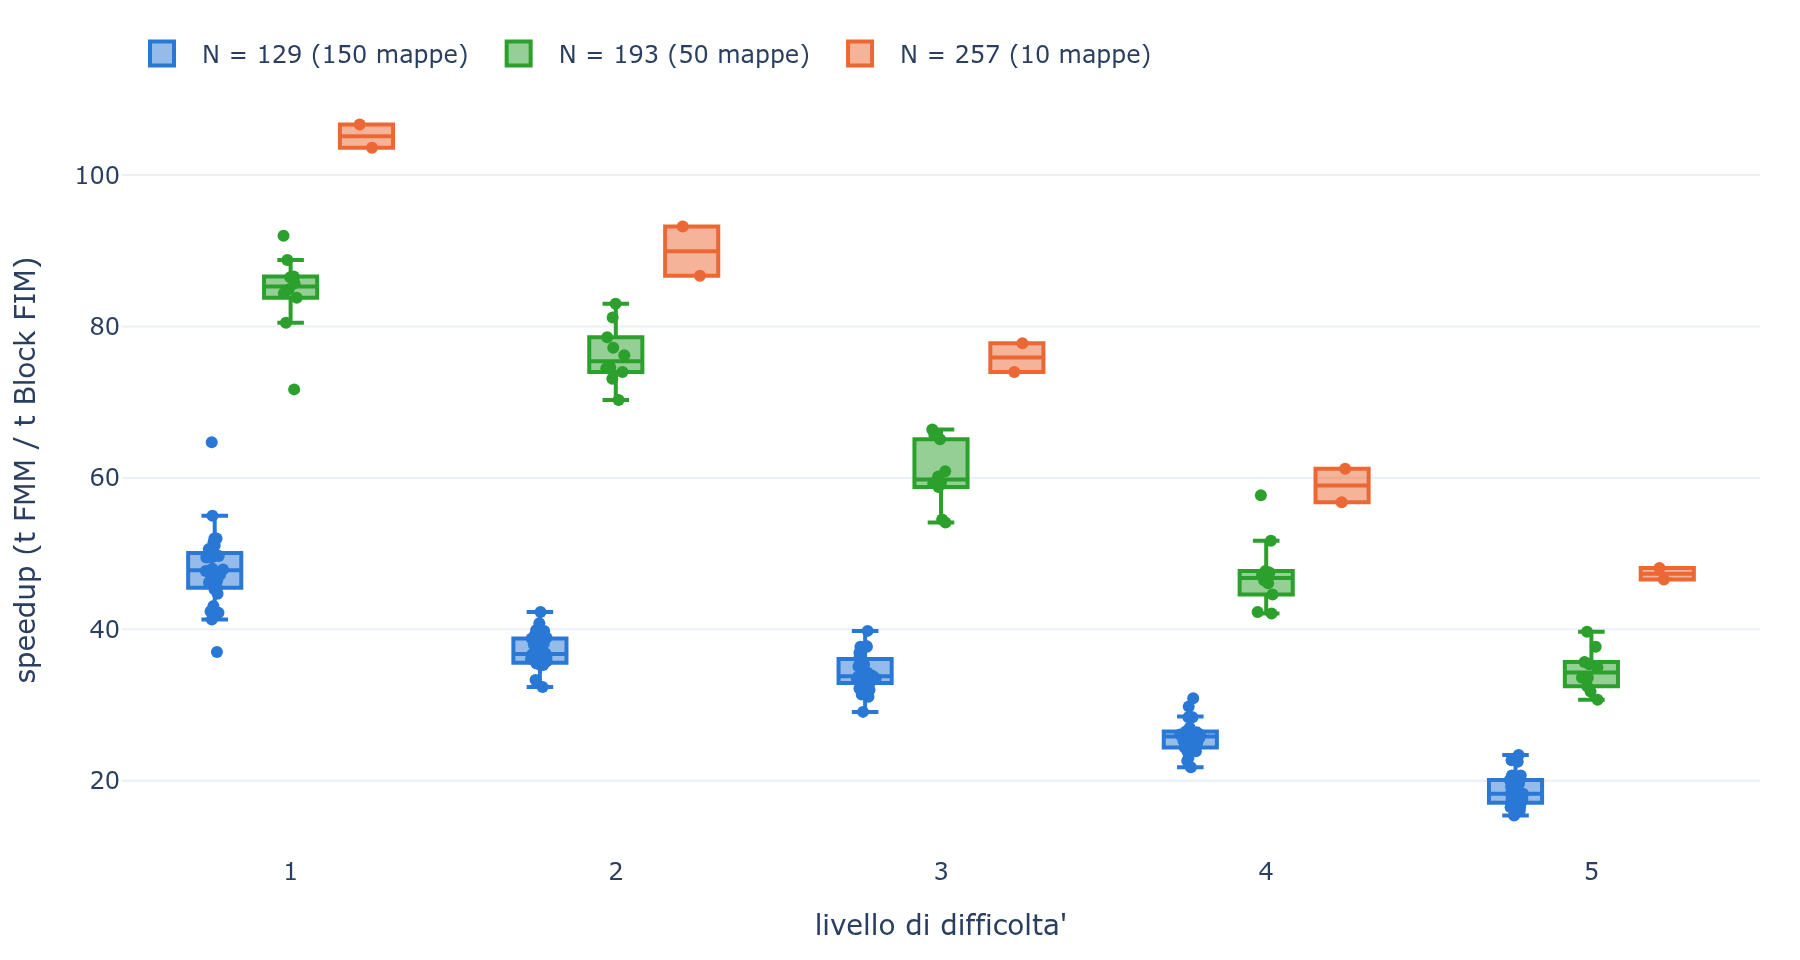
\includegraphics[width=\textwidth]{fig_speedup.png}
\caption{Speedup di ogni mappa (punti) e sua distribuzione (scatole), per livello e griglia.}
\end{figure}

\begin{figure}[H]
\centering
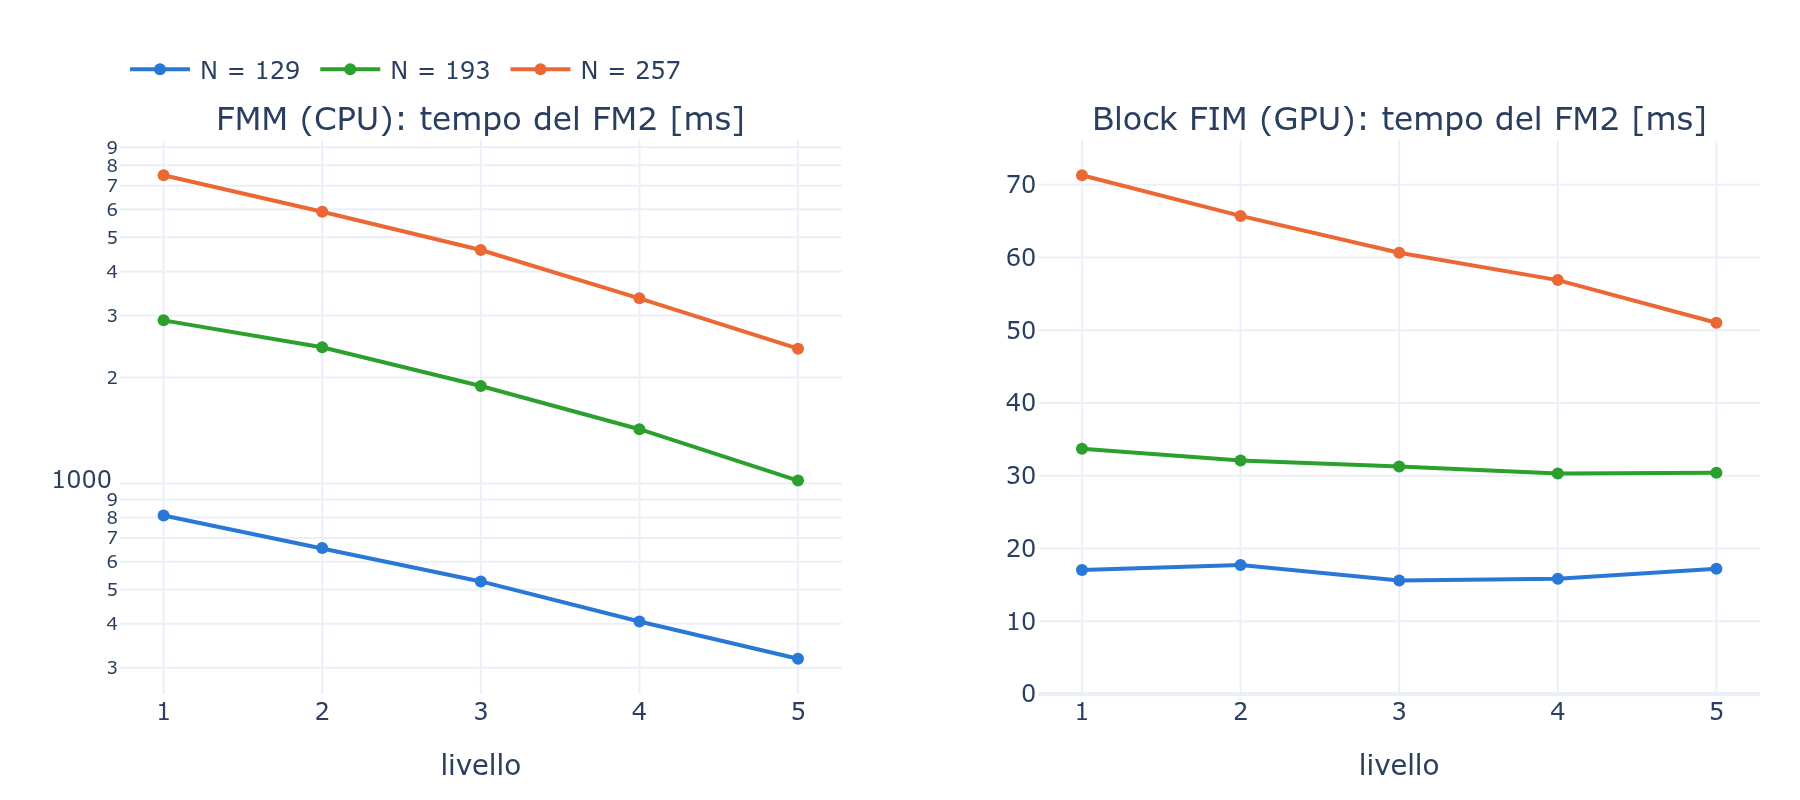
\includegraphics[width=\textwidth]{fig_tempi.png}
\caption{Tempo mediano del FM$^2$ per livello: FMM (scala logaritmica) e Block FIM.}
\end{figure}

\begin{figure}[H]
\centering
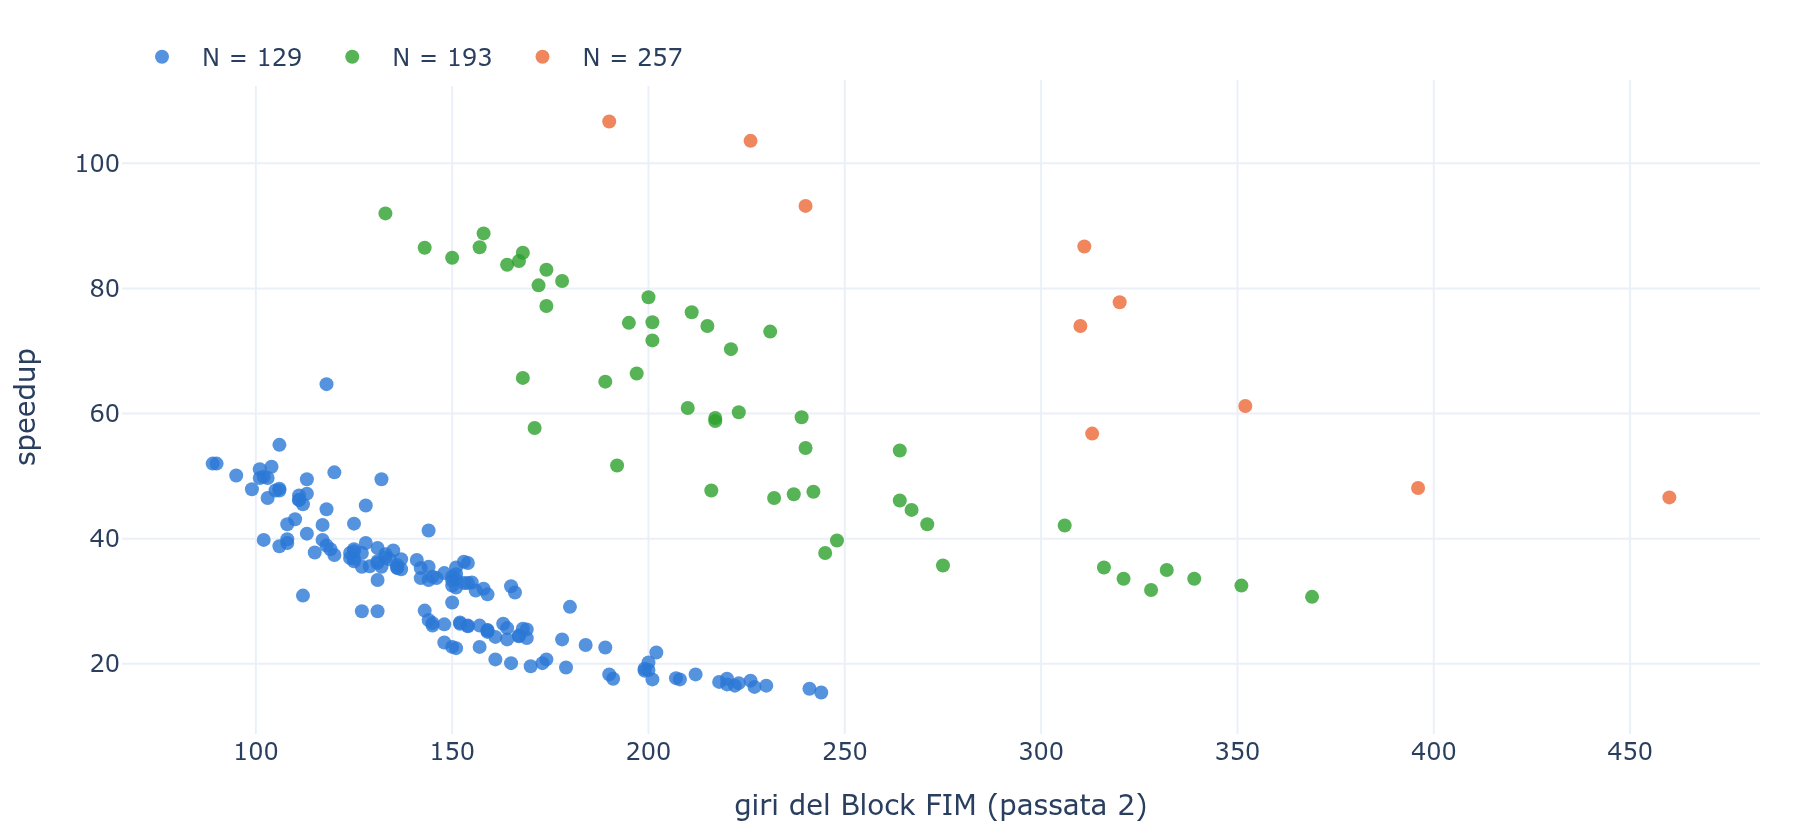
\includegraphics[width=\textwidth]{fig_giri.png}
\caption{Speedup contro numero di giri del Block FIM nella passata 2, mappa per mappa.}
\end{figure}

\section{Che cosa si osserva}
\begin{enumerate}
  \item \textbf{I due metodi danno la stessa soluzione.} Su tutte le 210 mappe la differenza massima tra le due $u$ è al più $1.1\cdot10^{-4}$, cioè al più $3.5\cdot10^{-6}$ volte $u(A)$: precisione della singola precisione (\texttt{float}). Il percorso del drone è quindi lo stesso; cambia solo il tempo per ottenerlo.
  \item \textbf{Il Block FIM è sempre più veloce}, in tutte le 210 mappe: lo speedup minimo è 15.4 ($N=129$, livello 5), il massimo 106.7 ($N=257$, livello 1). In valore assoluto il Block FIM resta sotto i 72 ms in tutte le prove; il FMM arriva a 7.6 s a $N=257$.
  \item \textbf{Lo speedup cresce con la griglia}, a ogni livello: al livello 1 passa da 48 ($N=129$) a 85 ($N=193$) a 105 ($N=257$); al livello 5 da 18 a 34 a 47. Più nodi ci sono, più la GPU è occupata in modo efficiente, mentre il FMM cresce più che linearmente con il numero di nodi.
  \item \textbf{Lo speedup cala con la difficoltà}, a ogni griglia: da 48 a 18 a $N=129$, da 85 a 34 a $N=193$, da 105 a 47 a $N=257$ (circa $2.2$--$2.6$ volte in meno dal livello 1 al livello 5).
  \item \textbf{Il calo viene soprattutto dal FMM che diventa più rapido, non dal Block FIM che rallenta.} Con più muri ci sono meno nodi liberi da calcolare (nelle mappe di prova a $N=129$: da $1.30\cdot10^6$ al livello 1 a $0.59\cdot10^6$ al livello 5, $-55\%$), e il tempo del FMM scende in proporzione ($-61\%$, da 811 a 318 ms). Il tempo del Block FIM invece resta quasi costante ($N=129$: 16--18 ms; $N=193$: 30--34 ms) o scende di poco ($N=257$: da 71 a 51 ms).
  \item \textbf{I giri del Block FIM crescono con la difficoltà} (a $N=129$ da 110 a 200 mediani; a $N=257$ da 208 a 428): il fronte deve girare attorno a più muri e passare per fori sfalsati, e i blocchi vengono riattivati più volte. Ogni giro però costa meno, perché i blocchi attivi per giro sono pochi (il fronte passa per fori stretti): il tempo per giro scende da 158 a 86 $\mu$s a $N=129$. I due effetti quasi si compensano.
  \item \textbf{A parità di livello, conta la forma del percorso.} Dentro uno stesso livello, le mappe con più giri hanno speedup minore (correlazione tra speedup e giri da $-0.8$ a $-0.9$ ai livelli 2--5): due mappe con le stesse regole ma con i fori più o meno allineati danno speedup diversi.
  \item \textbf{Le mappe difficili sono anche lente da volare}: il volo mediano passa da circa 23 s (livello 1) a circa 190--210 s (livello 5), perché il percorso è più lungo e il drone resta quasi sempre vicino ai muri, dove la velocità del FM$^2$ è bassa.
\end{enumerate}

\section{Limiti di questa prova}
\begin{itemize}
  \item A $N=257$ ci sono solo 2 mappe per livello: i valori indicano la tendenza, non una statistica.
  \item Il tempo del FMM è una sola misura per mappa; le misure ripetute negli altri notebook variano di pochi percento.
  \item Il tempo del Block FIM non comprende allocazione e copie tra CPU e GPU, come nelle altre tabelle.
  \item I tempi dipendono dalla GPU (Tesla T4) e dalla CPU assegnate da Colab.
  \item Il numero di nodi liberi per livello viene da una prova locale con gli stessi seed (la geometria non dipende dalla GPU); nel CSV di Colab è nella colonna
  \texttt{nodi\_liberi}.
\end{itemize}

\section{File}
\begin{itemize}
  \item \texttt{output\_colab\_2026-10-28.txt}: l'output completo della cella \texttt{!nvcc}.
  \item \texttt{risultati\_tutti.csv}: una riga per mappa (griglia, livello, seed, giri, differenza massima, $u(A)$, tempi, speedup).
  \item \texttt{fig\_speedup.png}, \texttt{fig\_tempi.png}, \texttt{fig\_giri.png}: le figure di questo documento.
\end{itemize}

\end{document}
